\documentclass[../main.tex]{subfiles}
\graphicspath{{\subfix{../images/}}}
\begin{document}
\section{Literature review}
\label{literature review}

The literature review for this thesis aims to provide an introduction and comprehensive overview of the
existing research on turn-taking in human robot interaction and the main methods used for the task of voice activity detection.

\subsection{Turn-taking in human robot interaction}
\label{turn-taking}

Turn-taking in the context of human communication and interaction is a highly complex and dynamic process rooted in sociolinguistics and cognitive psychology. It refers to the coordinated alternation of speaking and listening roles among participants engaged in conversation. This alternation is guided by a set of unwritten rules and social norms, often involving both verbal and non-verbal cues, which signal the transition between speaker and listener roles. Participants in a conversation constantly monitor these cues, including pauses, intonation patterns, and contextual information, to determine when it is appropriate to take the floor and contribute to the ongoing discourse. In human-robot interaction, replicating the intricacies of turn-taking is a significant challenge, as it involves programming robots to recognize and respond to these social cues and engage in conversational exchanges that align with human expectations. Achieving this capability is essential for creating socially competent and effective robotic systems that can seamlessly integrate into human social contexts.

In a recent article, "Turn-taking in Conversational Systems and Human-Robot
Interaction: A Review" \cite{skantze2021turn} is presented an overview of the fundamental concepts about turn-taking, the clues that have been found to facilitate turn-taking across different modalities, the techniques for the end-of-turn detection and prediction and other aspects of turn-taking in conversation systems that attracted some research in the last period. 

Starting from the fundamental concepts of turn-taking \cite{sacks1978simplest}, it can be analysed using units of speech called turn-constructional units (TCU) that are moments where an agent is considered the main speaker and the others are the listeners. Between TCUs there are transition-relevant places (TRP), where a turn shift generally happens. Inside the TCUs we can identify Inter-pausal units (IPUs), which are stretches of audio from one speaker without any silence exceeding a certain amount (such as 200ms). Generally we consider pauses silence between two IPUs within the same speaker and gaps IPUs between different speakers. In Figure \ref{fig:TPUs} is shown an example of conversation where the speaker is describing a route on a map to the listener. The figure shows also the principal components of the conversation in terms of units of speech. 

\begin{figure}[ht]
    \centering
    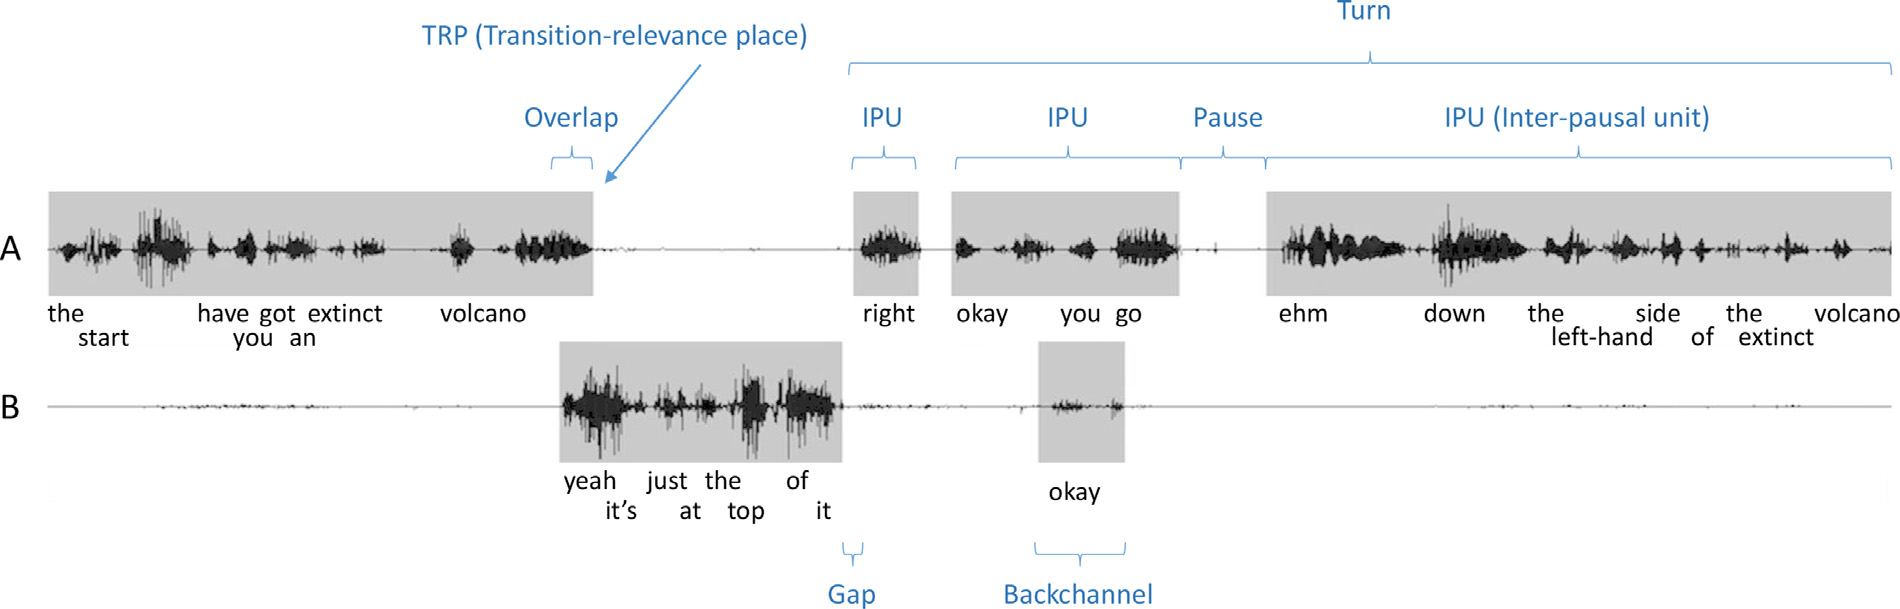
\includegraphics[width=\textwidth]{images/TPUs.png}
    \caption{Example of turn-taking and fundamental components \cite{anderson1991hcrc}.}
    \label{fig:TPUs}
\end{figure}


Regarding turn-taking cues, that can be divided in turn-yielding cues and turn-holding cues, the article underline how they do not have a specific effect on the listener, but they have an additive effect , where with the increase of turn-yielding cues, the listener was more incline to take the turn. 

The main turn-taking cues presented by the article are: 
\begin{itemize}
\item \textbf{Verbal cues}: "The completion of a syntactic unit is intuitively a requirement for considering the turn as “done” (a TRP)". Since syntactic and pragmatic completion can be very hard to determine, and that often it is important to consider the previous context, it is challenging to study the role of verbal cues in turn-taking.

\item \textbf{Prosody}: "Prosody refers to the non-verbal aspects
of speech, including intonation, loudness, speaking rate and timber. It has been found to serve many important functions in conversation, including the marking of prominence, syntactic disambiguation, attitudinal reactions, uncertainty, and topic shifts \cite{ward2019prosodic}". Generally , taking into consideration an English dialogue, it has been found that speakers approaching turn boundaries lower their voice intensity, whereas turn-internal pauses doesn't show this behaviour \cite{gravano2011turn}. Similar patterns were found in Japanese dialogue \cite{koiso1998analysis}, but different cultures and languages, for example Swedish \cite{edlund2005exploring}, can show differences.

\item \textbf{Breathing}: breathing is intrinsically linked to turn-taking because we typically breathe in before starting to speak. This means than an in-breath might serve as a turn-initial cue. A study on breathing in multi-party interactions \cite{ishii2014analysis} found that the speaker who holds the turn inhales more rapidly than when yielding the turn. Furthermore they found that the speaker who self-selected as the next speaker will take a deeper breath compared to listeners who are not about to speak, showing how breathe can help to coordinate self-selection in multi-party conversations. 

\item \textbf{Gaze}: "In face-to-face interaction, eye gaze has been found to serve many important communicative functions, including referring to
objects, expressing intimacy, dominance, and embarrassment, as well as regulating proximity and turn-taking". A study based on observations of recorded dyadic conversations \cite{kendon1967some} present a general pattern common to most of the conversations: at the start of the turn the speaker looks away, but then he shifts the gaze to the listener when the turn is ended and turn shift happens. Similarly the listener tends to look at the speaker for most part of the conversation while he tends to look away during turn shift when it is his turn to start speaking. Regarding multi-party interactions, gaze has an important role in the selection of the next speaker, where the current speaker will address the gaze towards the person he selected as the next speaker \cite{auer2018gaze}.

\item \textbf{Gestures}: in a study on turn-taking cues \cite{duncan1972some}, certain gestures seemed to be very effective as turn-holding cues, because the listener almost never attempted to take the turn during these type of gestures like tense hand position or movement away from the body. Another study on the role of gestures in language interaction \cite{holler2018processing} showed that questions accompanied by gestures resulted in faster response times compared to questions without gestures. So we can think that gestures help the listener to predict the end of a turn.

\end{itemize}

Regarding the end-of-turn detection and prediction models, which are the most studied aspect of turn-taking, their role is to understand when the user terminated his turn and the system can start to speak. End-of-turn detection is performed by the so called "reactive" models, because they tries do understand based on past clues if the turn is already ended. End-of-prediction, instead, is performed by the so called predictive models that tries to predict, base on the current clues, when the user is going to end the turn. In particular the article refer to three types of models, that are also shown in Figure \ref{fig:models}: 

\begin{figure}[ht]
    \centering
    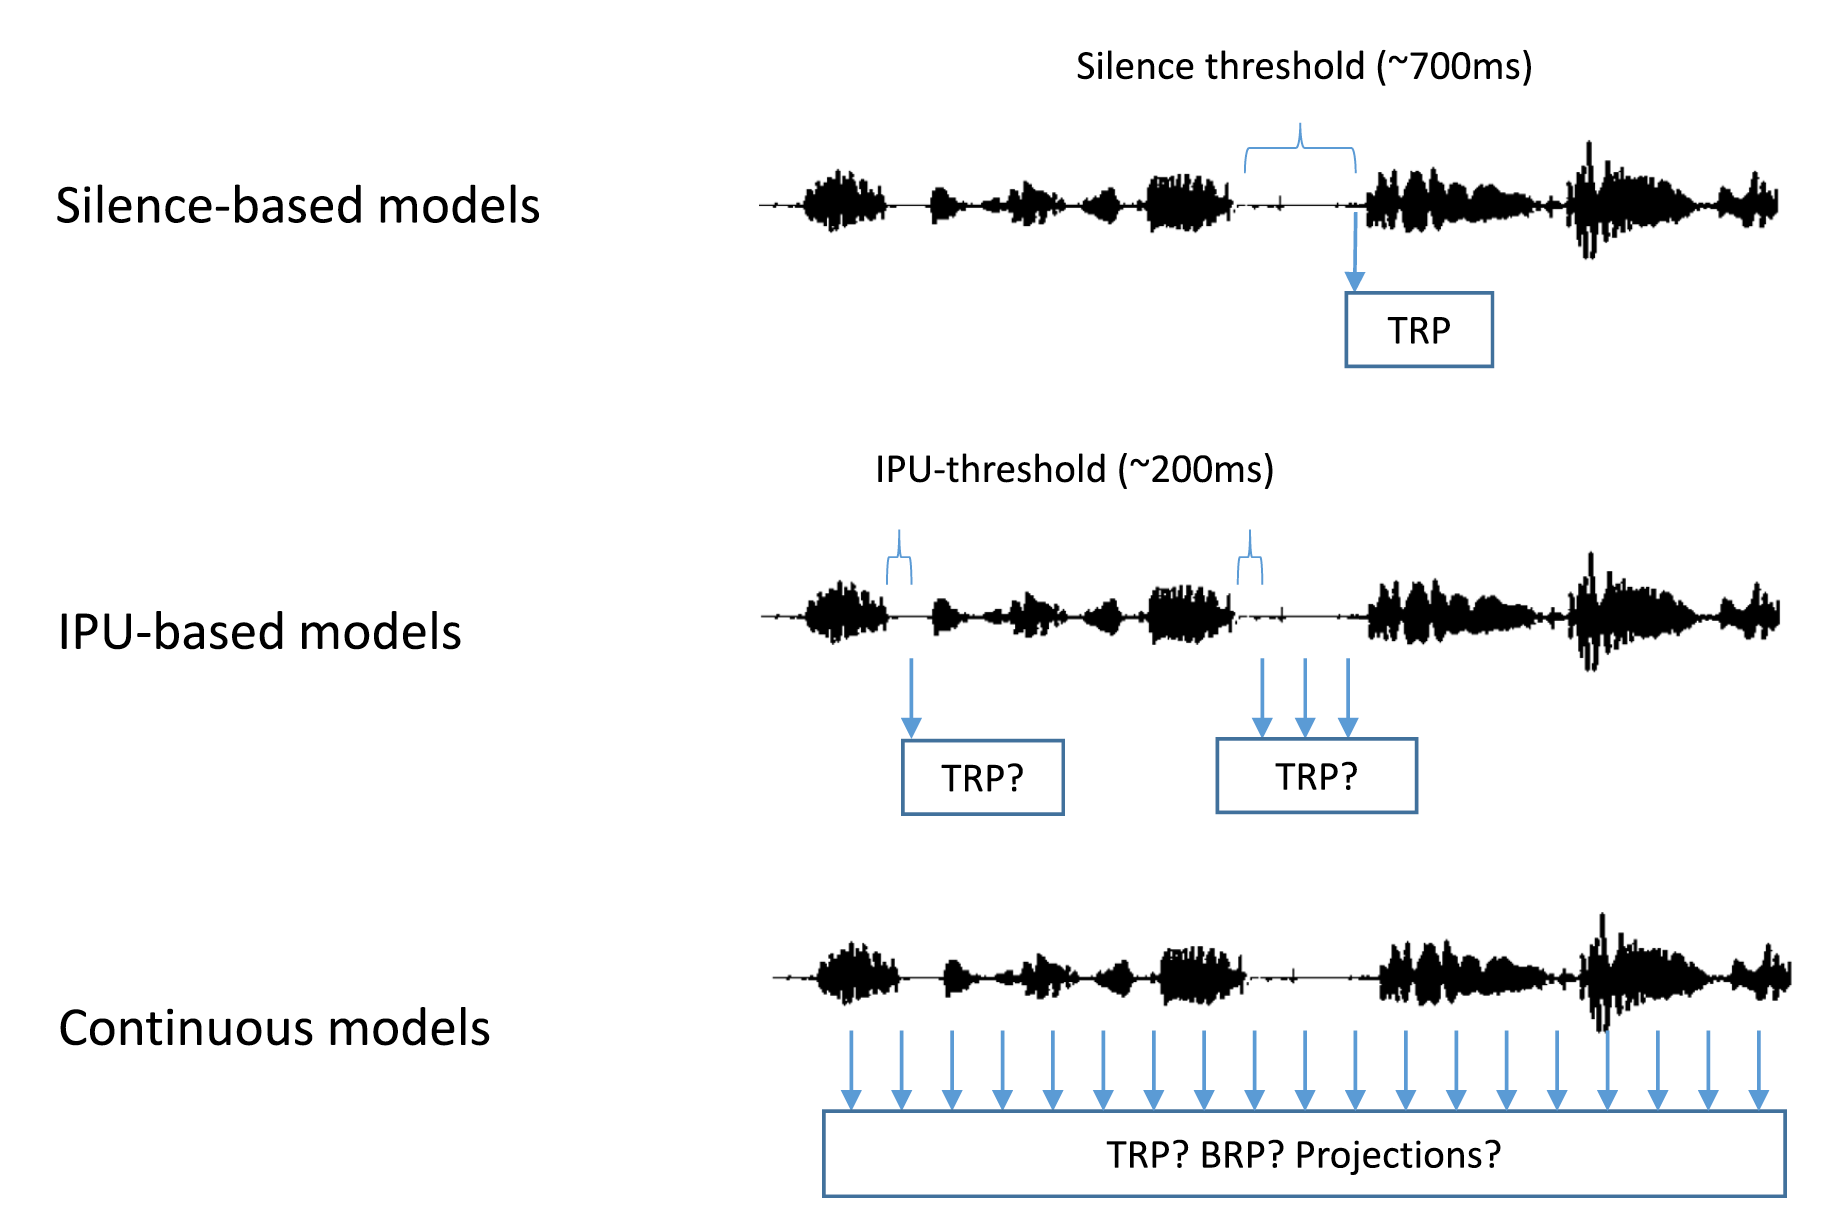
\includegraphics[width=\textwidth]{images/Turn-taking_models.png}
    \caption{Types of End-of-turn detection and prediction models \cite{skantze2021turn}}
    \label{fig:models}
\end{figure}

\begin{itemize}
\item \textbf{Silence-based models}: the end of the user’s turn is detected using a VAD, and a silence-threshold is used to understand when the turn is ended and the system can start to speak. “This approach is still being used in many conversational systems, and was for example assumed to be used in the VoiceXML standard, developed by W3C.”. Typically, some parameters (thresholds) can be tuned by the application developer, to regulate the turn-taking behaviour of the system.
This basic model is easy to implement and might work well in certain situations where the user knows what to say to the system. without uncertainty. On the other hand it presents 2 types of problems: if the turn-yielding threshold is too short, the system might misunderstand a user’s pause as an end of turn, while if it is too long the system will result unresponsive because it will have long response delays. To minimize these problems is important to tune these thresholds base on the use case application. The behaviour and possible problems of this model is shown in Figure \ref{fig:silence-based}.

\begin{figure}[ht]
    \centering
    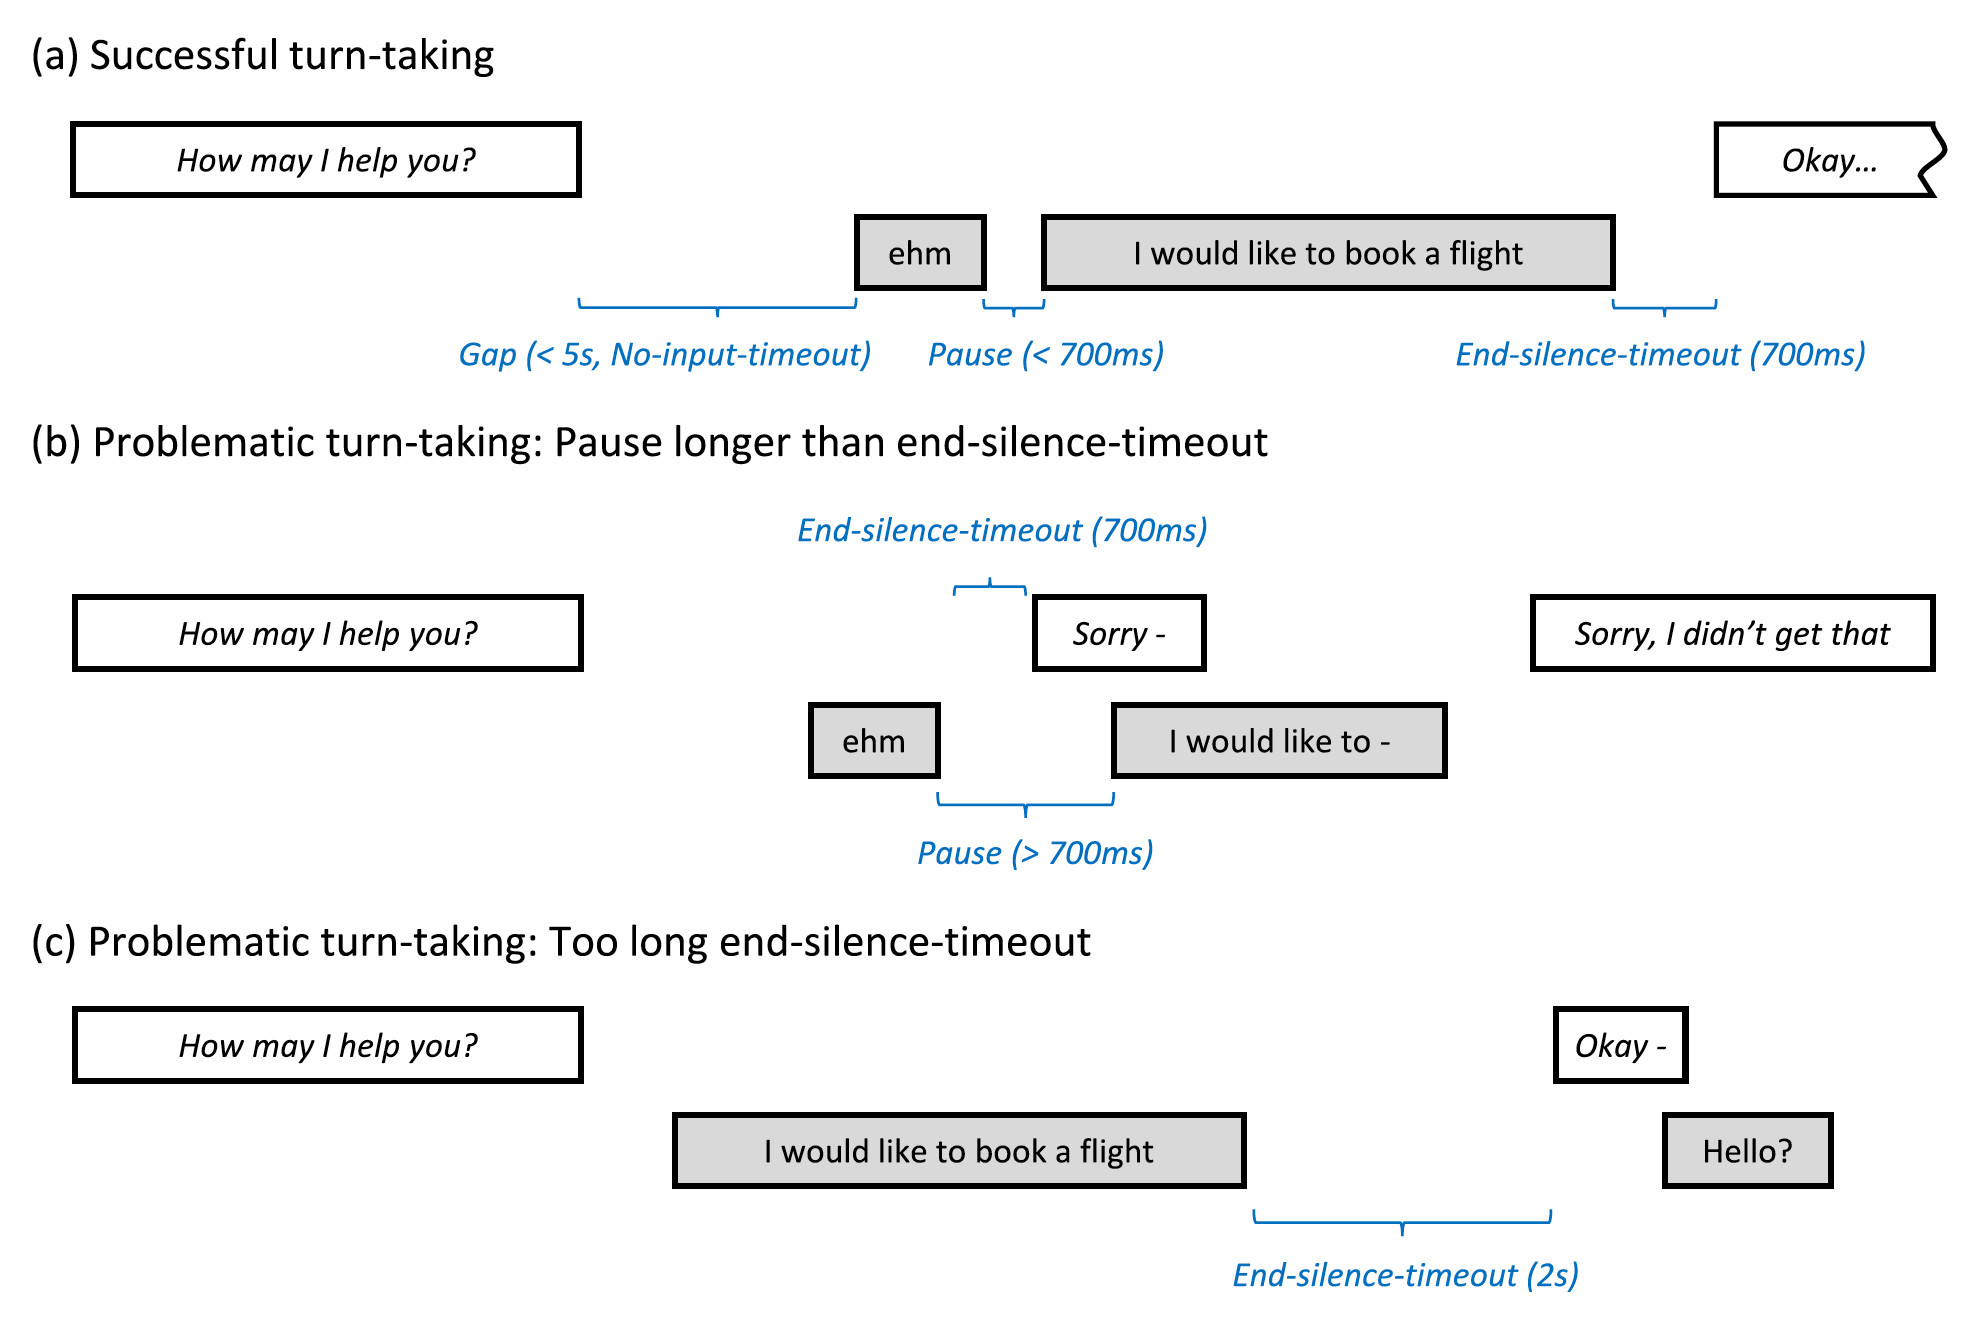
\includegraphics[width=\textwidth]{images/Silence-based model.png}
    \caption{Silence-based model \cite{skantze2021turn}}
    \label{fig:silence-based}
\end{figure}

\item \textbf{IPU-based models}: inter pausal units, that are potential turn-taking points, are detected using a VAD. Additionaly turn-taking cues in the user's speech are used to determine if the turn is ended or not. 

\item \textbf{Continuous models}: the user's speech is analyzed continuously to find possible points to take the turn. In this way the audio from the user is processed incrementally and all the models can start to process the input as soon as possible minimizing latency. Thus the system could also project turn completions. One of the main problems of these type of models is that they need constant revision, as what the system is understanding of what the user is saying my change with more speech. In this case the system processing might need a revision causing a cascade of revisions in the system that would increase latency.
\end{itemize}

\subsection{Voice activity detection (VAD)}
\label{voice activity detection}

Voice Activity Detection is a signal processing technique used to distinguish between segments of audio where speech is present and segments where there is no speech or background noise. It involves the analysis of audio signals to identify temporal regions during which a human speaker is actively speaking. VAD algorithms rely on various acoustic features and statistical methods to make this determination, and they are a fundamental component in applications like speech recognition, audio compression, and voice communication systems, where it's essential to focus processing and resources on speech segments while minimizing the impact of noise and silence.

VAD algorithms are typically made up of two processing stages: 

\begin{itemize}
    \item Features are extracted from noisy speech signal.
    \item A detection scheme is used on the feature to perform the classification.
\end{itemize}

Regarding classical VAD algorithms, the ones that do not use deep learning models to extract the features from the audio, an article by Simon Graf et al. \cite{graf2015features} presents what are the most used features extracted from the speech signal in order to perform the VAD activity:

\begin{itemize}
    \item \textbf{Energy}: it represents the power or intensity of an audio signal within a specific time frame. A common approach in VAD is to set an energy threshold. Frames with energy levels above this threshold are classified as speech, while those below it are classified as non-speech or noise. This is one of the simplest features taken into consideration. 

    \item \textbf{Zero-crossing rate}: It measures the rate at which the audio signal changes its sign or crosses the zero axis. Frames with zero-crossing rates above this threshold are more likely to be classified as speech, while frames with rates below it are more likely to be classified as non-speech or noise.  

    \item \textbf{Pitch and harmonicity}: this features analyse the pitch of the speech signal because it has been observed that voice produce an harmonically rich sound with a distinct pitch between 50 and 250 Hz. In particular Harmonicity measures the degree to which a sound is composed of harmonics, which are integer multiples of the fundamental frequency. Speech sounds are highly harmonic, meaning they contain a strong fundamental frequency and harmonics. Non-speech segments, on the other hand, tend to have lower harmonicity and more noise-like characteristics.

    \item \textbf{Formant structure}: The resonance frequencies, generated by the human vocal tract, results in a characteristic shape of the the spectral envelope. The Mel frequency cepstral coefficients (MFCCs), that rely on a transformation of the frequency axis, are computed. Finally, the cepstrum is calculated based on the modified spectrum.

    \item \textbf{Stationarity}: Speech signals are typically non-stationary. They exhibit variations in energy, pitch, and spectral content within short time frames. These variations are due to the dynamic nature of speech production, as speakers change their articulation, pitch, and loudness during conversation. In contrast, noise signals often exhibit more stationary characteristics. On the other hand background noise sources, tend to have relatively consistent statistical properties over short time frames. Under the assumption that noise is a stationary signal, the degree of non-stationarity can be employed for speech detection.

    \item \textbf{Modulation}: The temporal structure of speech is dominated by a characteristic
    energy modulation peak at about 4 Hz.This frequency corresponds to the typical syllable rate of human speech. Features that target at this property are robust against most interferences; however, a long window is necessary to capture it properly.

\end{itemize}

Classical VAD models use this extracted features in the detector module, where a fixed threshold is applied, to decide if the audio segment contains speech or not. Other important models for VAD are the statistical model-based approaches. This models uses the same features but extend the decision by prior knowledge of speech. The distributions of features for speech and noise are explicitly modeled by probability density functions. The choice of the model may vary, but common choices include Gaussian Mixture Models (GMMs) and Hidden Markov Models (HMMs).A threshold is now applied to the likelihood ratio of the speech and the noise model.

Another approach to perform voice activity detection is using neural networks. In a Google research article "Recurrent neural networks for voice activity detection" \cite{googleRNN} is presented a recurrent neural network (RNN) model for the VAD task. They present a multi-layer RNN model, in which nodes compute quadratic polynomials. The network outperforms a much larger baseline system composed of Gaussian mixture models (GMMs), that are statistical-model based algorithms. It uses one tenth the parameters and outperforms the GMM baseline system by 26\% reduction in false alarms, reducing overall speech recognition computation time by 17\%. Training was performed using supervised pairs of input and target output sequences of audio frames. The inputs are 13-dimensional PLP (Perceptual Linear Prediction) features, that are very similar to the features extracted with MFCC. 
 
\end{document}